\documentclass{article}
\usepackage[utf8]{inputenc}
\usepackage{hyperref}
\usepackage{graphicx}
\usepackage{float}
\usepackage{fancyhdr}

\usepackage{mathtools}
\renewcommand{\theequation}{eq. \arabic{equation}}


\usepackage[
  style=numeric,
  citestyle=numeric,
  url=false,
  doi=false,
  isbn=false
  ]{biblatex}
\addbibresource{main.bib}

\pagestyle{fancy}
\fancyhf{}
\rhead{Rikuo Hasegawa}
\lhead{UPCSE PHYSICS Long Lab Report}
\rfoot{p. \thepage}

\title{Random Article}
\author{ sp4ghet \\ Tutorial Group: aaa \\ Lab Pair: aaa \\ Lab Partners: aaa,\ aaa }

\begin{document}

\maketitle
\thispagestyle{fancy}
\newpage

\section*{Abstract}
  Random abstract \autocite{Hoge2017}
  \begin{equation}\label{eqn:euler}
    e^{i\pi} = -1
  \end{equation}
  \eqref{eqn:euler} is euler's formula \\
  $$ e^{i\theta} = \cos{\theta} + i\sin{\theta}$$
  is the more general formula

\section{Introduction}
aa

\subsection{Aims and Objectives}
aa

\subsection{Theory}
aa

\section{Experimental Equipment and Method}
aa

\subsection{Apparatus}
aa
\begin{figure}[H]
  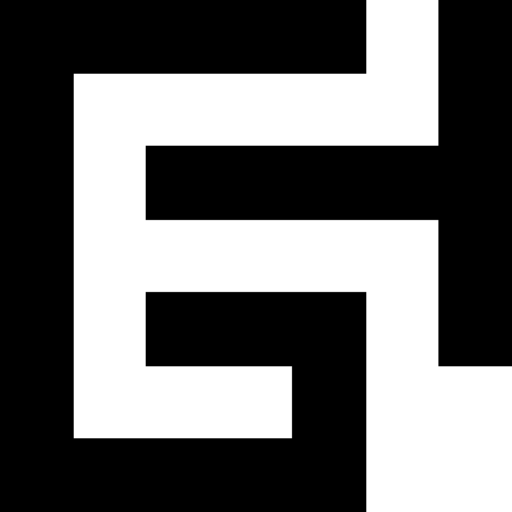
\includegraphics[width=\linewidth,natwidth=512,natheight=512]{img/hoge.png}
  \caption{Some Figure}
\end{figure}

\subsection{Method and Procedure}
aa

\section{Analysis of Results}
aa

\section{Discussion and Conclusion}
aa

\printbibliography
\end{document}
